\input devHead.tex
\SetTheme{AnnArbor} %10
\title{ソフトウェア開発\\第10回目授業}
\author{平野 照比古}
\institute{}
\date{2016/12/2}
\newtheorem{Prob}{解説}
\newcommand{\Elm}[1]{\texttt{<#1>}}
\setbeamercovered{transparent}

\newcommand{\DOMM}{\texttt}
\newcommand{\Event}{\texttt}
\newcommand{\DOMP}{\texttt}
\newcommand{\DOM}{\texttt{DOM}}
\newcommand{\keyitem}{\relax}
\newcommand{\HTML}{HTML文書}
\begin{document}
\frame{\maketitle}
%\frame{\tableofcontents}
\section{前回の演習問題}
\subsection{問題1}
\begin{frame}[containsverbatim]
 \frametitle{問題1}
 ルーブリックに記載したもの以外にもたくさんある。
\begin{center}
 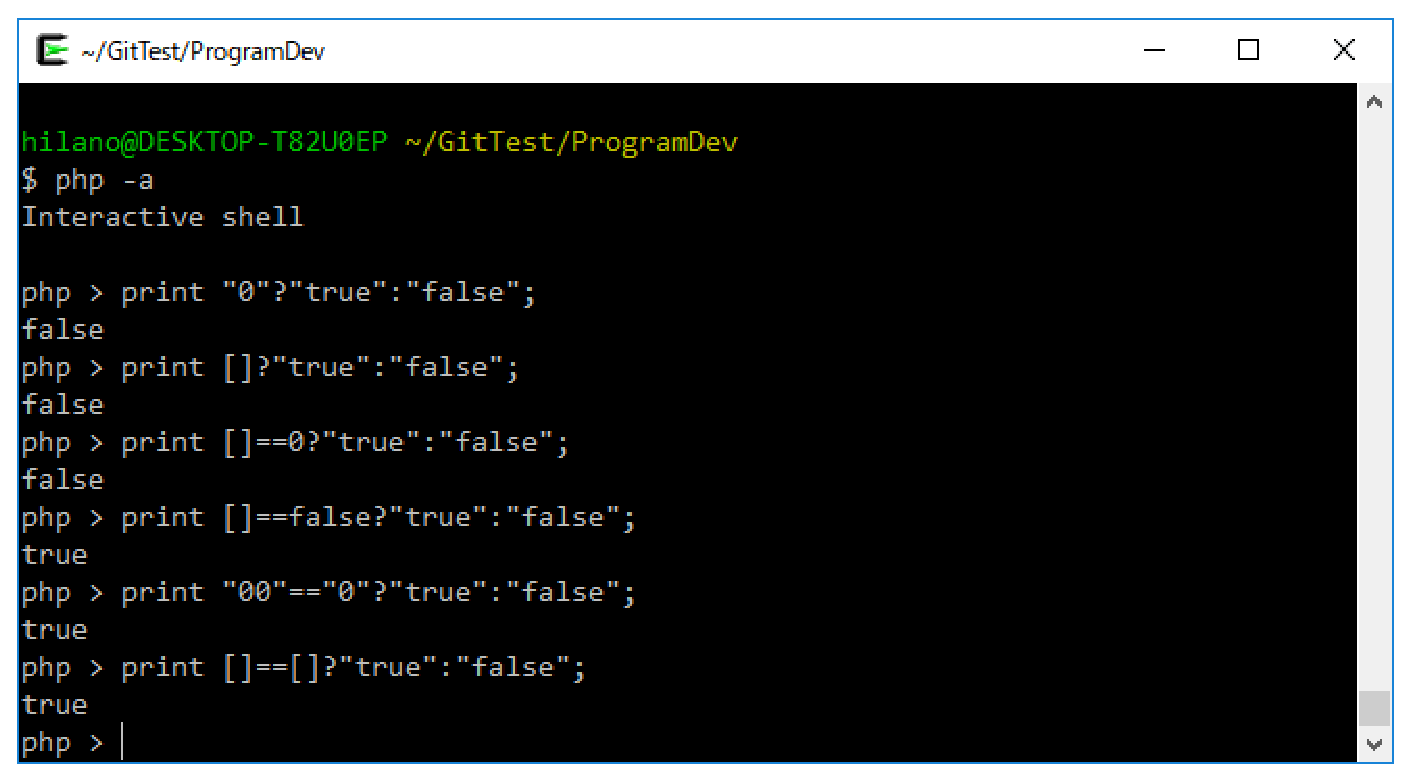
\includegraphics[width=0.8\textwidth]{09-01fig-result1.eps}
\end{center}
\end{frame}
\subsection{問題2}
\begin{frame}[containsverbatim]
 \frametitle{問題2}
 \begin{Verbatim}
	$a = array(1,2,3,"4");
 \end{Verbatim}
 とおいて違いを見るとよい。

 ブラウザで実行した場合には、表示された画面のソースを見るほうが結果が見
 やすい。
\end{frame}
\begin{frame}[containsverbatim]
 \frametitle{問題3--\Verb+array\_splice()+の仕様}

 \Verb+array array_splice ( array &$input , +\\
 \Verb+int $offset [, int $length = count($input)+
 \Verb+[, mixed $replacement = array() ]] )+
 \begin{itemize}
  \item input 入力の配列。
  \item offset offset が正の場合、削除される部分は 配列 input の最初から
        指定オフセットのぶんだけ進んだ位置\\
        offset が負の場合、削除される部分は、 input の末尾から数えた位置
  \item length length が省略された場合、 offset から配列の最後までが全て
        削除\\
        length が指定され、正の場合、複数の要素が削除\\
        負の length が指定された場合、削除される部分の末尾の位置は配列の
        末尾を基準にして計算されます。\\
        length にゼロを指定した場合は、どの要素も削除しません。
  \item replacement
配列 replacement が指定された場合、 削除された要素は、この配列の要素で置換
 \end{itemize}
\end{frame}
 \begin{frame}[containsverbatim]
  \frametitle{問題2}
  \LISTNN{09pop-push.php}{1}{last}{\small}
 \end{frame}
\subsection{問題3}
 \begin{frame}[containsverbatim]
  \frametitle{問題3}
  \VerbatimInput[fontsize=\scriptsize]{../09testPHP.php}
 \end{frame}
 \begin{frame}[containsverbatim]
  \frametitle{問題3--結果}
  \begin{itemize}
   \item PHPでは\texttt{+}数として加法
   \item 文字列は数として正しいところまで変換
   \item \texttt{1:}では\"内の変数は値に置き換えられる
   \item \texttt{2:}では\Verb+"2:"+の部分は数の$2$に変換、その後加法が行
         われ、$9$となる。改行コードは数の$0$に変換
   \item \texttt{3:}では\Verb+"3:".$A+の部分は\Verb+"3:2"+になり、
         \texttt{+}で$3+5$が計算される。
   \item PHPでは引数が少ないと警告が出る。多い方は無視
   \item \Verb+sum2()+内では\Verb+$A+などは関数内で値が定義されていない
         ので警告が出る
  \end{itemize}
 \end{frame}
 \begin{frame}[containsverbatim]
  \frametitle{}
 \end{frame}
\section{PHP入門--続き}
 \input dev2016-09php2.tex
\section{サーバーとのデータ-の交換(1)}
% \subsection{サーバーとのデータのやり取り}
 \begin{frame}[containsverbatim]
 \frametitle{サーバーとのデータ交換の基本}
 Webページにおいてサーバーにデータを送る方法には\texttt{POST}と
 \texttt{PUT}の2通りの方法がある。
 \end{frame}
 \begin{frame}[containsverbatim]
 \frametitle{\texttt{POST}による送信}
 \texttt{windows.onload =function()}内に次のコードを追加する。
 \begin{Verbatim}
    let Form = document.getElementsByTagName("form")[0];
    Form.setAttribute("method","POST");
    Form.setAttribute("action","09sendData.php");
 \end{Verbatim}
 HTMLの要素に対しては次のことを行う。
 \begin{itemize}
 \item \texttt{<select>}要素の属性に\verb+name="select"+ を追加する。
 \item \texttt{id}が\verb+"colorName"+であるテキストボックスに
       \verb+name="colorName"+ を追加する。
 \item 「設定」ボタンの要素の後に次の要素を追加する。
 \begin{center}
 \verb+<input type="submit" value="送信" id="Send"></input>+ 
 \end{center}
 \end{itemize}
 一時期は\texttt{name}属性を指定しておくと、\texttt{id}属性を兼ねていた時
 期もあったが、最近では両者は厳密に区別されている。
\end{frame}
 \begin{frame}[containsverbatim]
 \frametitle{\texttt{POST}による送信(解説)}
 \begin{itemize}
 \item このページでは「送信」ボタンを押すと\texttt{<form>}の
 \texttt{action}属性で指定されたプログラムが呼び出される。
 \item ここではWebペー ジと同じ場所にある\texttt{09sendData.php}が呼び出
      される。
 \end{itemize}
 \end{frame}
 \begin{frame}[containsverbatim]
 \frametitle{サーバープログラムのリスト}
 \begin{Verbatim}[numbers=left, fontsize=\scriptsize]
 <?php
 print <<<_EOL_
 <!DOCTYPE html>
 <head>
 <meta charset="UTF-8"/>
 <title>サーバーに送られたデータ</title>
 </head>
 <body>
 <table>
 _EOL_;
 foreach($_POST as $key=>$value) {
  print "<tr><td>$key</td><td>$value</td></tr>\n";
 }
 print <<<_EOL_
 </table>
 </body>
 </html>
 _EOL_;
 ?>
 \end{Verbatim}
 \end{frame}
 \begin{frame}[containsverbatim]
 \frametitle{サーバープログラムのリスト(解説)}
 \begin{itemize}
 \item 2行目から10行目の間はヒアドキュメント形式でHTML文書の初めの部分を
       出力させている。
 \item \verb+method="POST"+で呼び出されたときには\texttt{form}要素内の
       \texttt{name}属性が指定されたものの値がスーパーグローバル
       \verb+$_POST+内の連想配列としてアクセスができる。
 \item 11行目から13行目でそれらの値を\texttt{table}要素内の要素として出
       力している。
 \end{itemize}
 \end{frame}
 \begin{frame}[containsverbatim]
 \frametitle{サーバープログラムのリスト(ソース)}
 \begin{Verbatim}
 <!DOCTYPE html>
 <head>
 <meta charset="UTF-8"/>
 <title>サーバーに送られたデータ</title>
 </head>
 <body>
 <table><tr><td>select</td><td>yellow</td></tr>
 <tr><td>color</td><td>green</td></tr>
 <tr><td>colorName</td><td>gray</td></tr>
 </table>
 </body>
 </html>
 \end{Verbatim}
 \end{frame}
 \begin{frame}[containsverbatim]
 \frametitle{\texttt{GET}による通信}
 \begin{itemize}
 \item \Verb+method="PUT"+で呼び出した場合にはスーパーグローバル
 \Verb+$_GET+を用いる。
 \item スーパーグローバル\Verb+$_REQUEST+は
 \Verb+method="POST"+でも\Verb+method="PUT"+で呼び出された場合の
 \Verb+$_POST+や\verb+$_GET+の代わりに使用できる。
 \end{itemize}
 \end{frame}
 \begin{frame}[containsverbatim]
 \frametitle{通信に関する注意}
 \begin{itemize}
 \item \Verb+type="submit"+の\texttt{input}要素は、ボタンが押されたときに直ちに、
 \texttt{action}属性で指定された処理が呼び出される。
 \item サーバーにデータを送る前に最低限のエラーチェックを行い、エラーが
       ない場合にだけサーバーと通信するのが良い。
 \end{itemize}
 \end{frame}
 \begin{frame}[containsverbatim]
 \frametitle{スパーグローバルの補足}
 \begin{itemize}
 \item {\texttt{\$\_SERVER}}\\
 サーバーにアクセスしたときのクライ
 アントの情報などを提供。具体的な内容はクライアントごとに異なる。
 \item \texttt{\$\_COOKIE}\\
 COOKIE とはWebサーバー側からクライアント側に一時的にデータを保存させる仕
 組み。すでに訪問したことがあるサイトに対して情報を開始
 時に補填する機能などを実現できる。
 \item \texttt{\$\_SESSION}\\
 セッションとはある作業の一連の流れを指す。たとえば会員制のサイトではログイ
 ン後でなければページを見ることができない。情報のページに直接行くことがで
 きないような仕組みが必要
 \end{itemize}
 \end{frame}
 \begin{frame}[containsverbatim]
 \frametitle{セッション}
 \begin{itemize}
 \item HTTP通信はセッションレスな通信である(各ページが独立して存在し、ページ間
 のデータを直接渡せない)
 \item セッションを確立するためには、クライアント側から情報を送り、それに基づい
 てサーバー側が状況を判断するなどの操作を意識的にする必要
 \item PHPではセッションを開始するための関数\texttt{session\_start()}とセッショ
 ンを終了させる\texttt{session\_destroy()}が用意されている。
 \item セッションを通じで保存させておきたい情報はこの連想配列に保存
 \item セッションの管理はサーバーが管理
 \item この機能はCOOKIEの機能を利用して実現
 \end{itemize}
 \end{frame}
 \section{Web Storage}
\begin{frame}[containsverbatim]
 \frametitle{Web Storage}
 \begin{itemize}
 \item localStoarage と sessionStorage の2種類
 \item localStorage は文字列をキーに、文字列の値を持つStorageオブジェク
 ト
 \item 同一の出身(プロトコルやポート番号も含む)のすべてのドキュメント
 がおなじlocalStorageを共有
 \item このデータは意識的に消さない限り存在
 \item sessionStorageはウインドウやブラウザが閉じられると消滅
 \item セッション間の情報の移動を可能にしている。
 \end{itemize}
 \end{frame}
 \begin{frame}[containsverbatim]
 \frametitle{Web Storageの補足}
 \begin{itemize}
 \item いくつかのサイトではこの機能を用いており、その開発者ツールで見る
       ことが可能
 \item データの形式は文字列である。構造化されたデータはJSON形式で保存するのがよい
 \end{itemize}
 \end{frame}
\begin{frame}[containsverbatim]
 \frametitle{WebStrageの例(1)}
 \begin{Verbatim}[fontsize=\small]
<!DOCTYPE html>
<html>
<head>
<meta http-equiv="Content-Type" content="text/html; charset=utf-8"/>
<title>WebStorage --- localStorage</title>
\end{Verbatim}
 \end{frame}
\begin{frame}[containsverbatim]
 \frametitle{WebStrageの例(2)}
  \begin{Verbatim}[numbers=left, fontsize=\scriptsize]
<script type="text/javascript">
//<![CDATA[
var Storage = window.localStorage;
//var Storage = window.sessionStorage;
window.onload = function() {
  let AccessList, Message = document.getElementById("message");
  let D = new Date();
  if(Storage["access"]) {
    AccessList = JSON.parse(Storage["access"]);
  } else {
    AccessList = [];
    appendMessage(Message, "初めてのアクセスです");
  }
  AccessList.unshift(D.getTime());
  Storage["access"] = JSON.stringify(AccessList);
  appendMessage(Message, "今までのアクセス時間です");
  AccessList.forEach(function(D, i, A) {
    appendMessage(Message, new Date(D));
  });
}
\end{Verbatim}
 \end{frame}
\begin{frame}[containsverbatim]
 \frametitle{WebStrageの例(3)}
  \begin{Verbatim}[numbers=left, fontsize=\small]
function appendMessage(P, Mess) {
  let div = document.createElement("div");
  P.appendChild(div);
  div.appendChild(document.createTextNode(Mess));
}
//]]
</script>
</head>
 \end{Verbatim}
\end{frame}
\begin{frame}[containsverbatim]
 \frametitle{WebStrageの例(4)}
  \begin{Verbatim}[numbers=left, fontsize=\small]
<body>
  <form action="10next.html">
    <input type="submit" value="次のページ"></input>
  </form>
  <div  id="message"/>
</body>
</html>
\end{Verbatim}
\end{frame}
\section{サーバーとのデータ-の交換--Ajax}
\subsection{Ajax}
\begin{frame}[containsverbatim]
\frametitle{Ajax\footnote{Ajaxの名称を提案したブログ
 \texttt{http://adaptivepath.org/ideas/ajax-new-approach-web-applications/}}
 とは}
\begin{itemize}
 \item Asynchronous Javascript+XML の略
 \item 非同期(Asynchronous)でWeb
ページとサーバーでデータの交換を行い、クライアント側で得られたデータをも
とにそのWebページを書き直す手法
\end{itemize} 

\begin{itemize}
 \item Google Maps がこの技術を利用したことで一気に認知度が高まった。
 \item 検索サイト
では検索する用語の一部を入力していると検索用語の候補が出てくる。これも
Ajaxを使用している(と考えられる)。
\end{itemize}
\end{frame}
\begin{frame}[containsverbatim]
\frametitle{\texttt{XMLHTTPRequest}}
Ajax の機能はこのオブジェクトを用いて実現

\begin{itemize}
 \item 日付が変わったときに、その日の記念日を
 メニューの下部に示す
 \item 記念日のデータは
 \texttt{http://ja.wikipedia.org/wiki/日本の記念日一覧}の表示画面からコ
 ピーして作成
\end{itemize}
\end{frame}
\begin{frame}[containsverbatim]
\frametitle{リスト(1)}
\LISTNN{09-01whatday.html}{42}{48}{\normalsize}
\end{frame}
\begin{frame}[containsverbatim]
\frametitle{リスト---概要}
\begin{itemize}
 \item 以前のものとは41行目から61行目が異なっている。
 \item イベントハンドラーを関数として定義している。
 \item 42行目から48行目は以前と同じプルダウンメニューの処理である。
\end{itemize}
\end{frame}
\begin{frame}[containsverbatim]
\frametitle{リスト(2)--- XMLHttpRequestオブジェクトの生成}
\LISTNN{09-01whatday.html}{49}{63}{\small}
\end{frame}
\begin{frame}[containsverbatim]
\frametitle{\texttt{XMLHttpRequest}の作成}
49行目でサーバーと通信をするための
\texttt{XMLHttpRequest}オブジェクトを作成している。
\end{frame}
\begin{frame}[containsverbatim]
\frametitle{リスト(3)--- コールバック関数の登録}
\LISTNN{09-01whatday.html}{51}{56}{\scriptsize}
\end{frame}
\begin{frame}[containsverbatim]
\frametitle{イベントハンドラーの説明}
\texttt{XMLHttRequest}が生成できていたら(50行目)、このオブジェクトが
       生成する\texttt{onreadystatechange}イベントのイベントハンドラーを
       登録する(51行目から56行目)。
 \begin{itemize}
  \item \texttt{XMLHttRequest}の\texttt{readyState}は通信の状態を表す。
	$4$ は通信終了を意味する。
  \item 通信が終了しても正しくデータが得られたかを調べる必要がある。
	$200$ は正しくデータが得られたことを意味する。
  \item 得られたデータは\texttt{responseText}で得られる。この場合、得ら
	れたデータは文字列となる。このほかに\texttt{responXML}でXMLデー
	タが得られる。
 \end{itemize}
%\end{frame}
%\begin{frame}[containsverbatim]
\frametitle{通信の開始}
\begin{itemize}
 \item 57行目から59行目が通信の開始する。ここでは、\texttt{GET}で行うので、
       URLの後に必要なデータを付ける。
 \item \texttt{GET}では送るデータ本体がないので、通信の終了をのため
       \texttt{null}を送信する。\texttt{POST}のときはここでデータ本体を
       送る。
 \item プルダウンメニューが変化したときのイベントハンドラーを登録し(62行
       目)、最後に現在の日付データをサーバーに要求する。、
\end{itemize}
\end{frame}
\begin{frame}[containsverbatim]
\frametitle{リスト(4)---HTML文書}
\LISTNN{09-01whatday.html}{63}{71}{\normalsize}
\end{frame}
\begin{frame}[containsverbatim]
\frametitle{送られてきたデータの処理}
\begin{itemize}
 \item 得られたデータは70行目の\texttt{p}要素の中に入れる(53行目から54行
       目)。
 \item この要素の\texttt{firstChild}を指定しているので85行目には
       \texttt{<p>}と\texttt{</p>}の間に空白を設けて、テキストノードが存
       在するようにしている。
\end{itemize}\end{frame}
\begin{frame}[containsverbatim]
\frametitle{Ajaxで呼び出されるPHPのプログラム}
\LISTNN{aniversary.php}{1}{last}{\scriptsize}
\end{frame}
\begin{frame}[containsverbatim]
\frametitle{Ajaxで呼び出されるPHPのプログラム--解説}
\begin{itemize}
 \item 2行目で内部で処理をするエンコーディングを\texttt{UTF8}にしている。
       関数、\texttt{mb\_internal\_encoding}関数を引数なしで呼び出すと
       現在採用されているエンコーディングを得ることができる。
 \item 4行目と5行目では月(\verb+$m+)と日(\verb+$d+)の値をそれぞれの変数
       に設定している。
\begin{itemize}
 \item ここではコマンドプロンプトからもデバッグで
       きるように、スーパーグローバル\verb+$_GET+内に値があれば
       (\Verb+isset()+)が\Verb+true+になれば、その値を、そうでなければコ
       マンドからの引数を設定している。
 \item スーパーグローバル\verb+$argv+はの先頭は呼び出したファイル名であ
       り、その後に引数が順に入る\footnote{C言語の\texttt{main}関数は通
       常、\texttt{int main(int argc, char* argv[])}と宣言される。%
       \texttt{argc}は\texttt{argv}の配列の大きさを表し、渡された引数の
       リストが\texttt{argv[]}に入っている。このとき、\texttt{argv[0]}は実行
       したときのファイル名が入る。}。
\end{itemize}
\end{itemize}
\end{frame}
\begin{frame}[containsverbatim]
\frametitle{\texttt{file()}関数}
指定されたファイルを行末文字で区切って配列として返す関数\\
\begin{itemize}
\item 引数にはURLも指定できる。
\item この関数は2番目の引数をとることができる。
\begin{center}
 \begin{tabular}{|c|m{15zw}|}\hline
 \Verb+FILE_USE_INCLUDE_PATH+ & \Verb+include_path+ のファイルを探す\\\hline
 \Verb+FILE_IGNORE_NEW_LINES+ & 配列の各要素の最後に改行文字を追加しない
      \\ \hline
  \Verb+FILE_SKIP_EMPTY_LINES+&空行を読み飛ばす \\ \hline
 \end{tabular}
\end{center}
 \item \verb+file_get_contents()+はファイルの内容を一つの文字列として
       読み込む。Webページの解析にはこちらの関数を使うとよい。
\end{itemize}
\end{frame}
\begin{frame}[containsverbatim]
\frametitle{読み込むファイルの一部}
\begin{Verbatim}
1月[編集]
1日 - 鉄腕アトムの日
2日 - 月ロケットの日
[中略]
31日 - 生命保険の日、愛妻家の日
2月[編集]
1日 - テレビ放送記念日、ニオイの日
2日 - 頭痛の日
[以下略]
\end{Verbatim}
\end{frame}
\begin{frame}[containsverbatim]
\frametitle{}
\begin{itemize}
 \item 月の部分の後には\texttt{[}がある。
 \item 日の情報は\verb*+ - +で区切られている(\verb*+ +は空白を表す)。
 \item すべての日の情報が入っている。
\end{itemize}
\end{frame}
\begin{frame}[containsverbatim]
\frametitle{データの処理---月を探す}
\begin{itemize}
 \item 8行目で念のためコードを\texttt{UTF8}に変更
 \item 関数\Verb+mb_split()+関数は第1引数に指定された文字列パターンで第2
       引数で指定された文字列を分割して配列として返す関数
 \item 分割を指定する文字列には正規表現が使えるので、文字\Verb+[+で分割
       するために、\Verb+"\["+としている(9行目)。
 \item 指定された文字列があれば配列の大きさが1より大きくなる。その行に対
       して求める月と一致しているか判定し、等しければループを抜ける(11行
       目)。
\end{itemize}
\end{frame}
\begin{frame}[containsverbatim]
\frametitle{}
\begin{itemize}
 \item 14行目から18行目までは指定された月での指定された日の情報を探して
       いる。日を決定する方法も月と同じである。文字列の分割は
       \verb+"\s-\s"+となっている\footnote{これは\texttt{"\textbackslash
       s"}ではうまく行かなかっ
       たためである。}。
 \item 20行目で得られた情報をストリームに出力している。
\end{itemize}
\end{frame}
\end{document}
